\section{Analyse des Krebsnebels}
\label{sec:analyse}

\subsection{Ablauf einer stereoskopischen MAGIC Analyse}

\begin{figure}
  \centering
  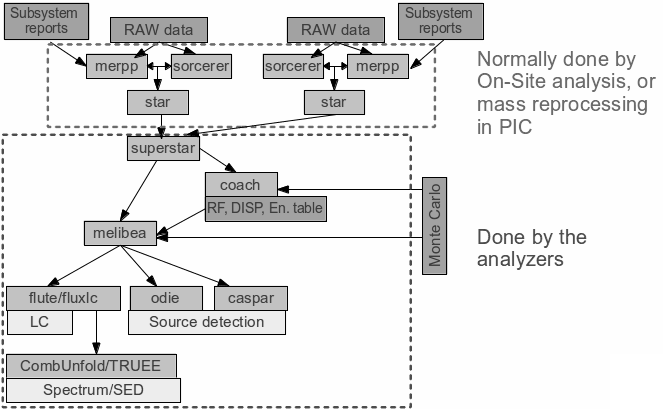
\includegraphics[width=0.9\textwidth]{figures/analysischain.png}
  \caption{Ablauf einer typischen stereoskopischen Analyse. Zunächst werden die
  Rohdaten der beiden Teleskope einzeln vorprozessiert und dann durch die
  Software superstar kombiniert. [...]}
  % Referenz: MAGIC wiki
  \label{fig:analysis_chain}
\end{figure}

\subsection{Wahl der Analyseparameter}

\subsection{Ergebnisse}
